\documentclass{article}

\usepackage[top=5cm, bottom=5cm, left=3.5cm, right=3.5cm]{geometry}
\usepackage[german]{babel}
\usepackage{xspace}
\usepackage{hyperref}
\usepackage{graphicx}
\usepackage[np]{numprint}
\usepackage{listings}
\usepackage{color}

\newcommand{\wow}{World of Warcraft\xspace}
\newcommand{\mpq}{MoPaQ\xspace}
\newcommand{\blizzard}{Blizzard\xspace}
\newcommand{\file}[1]{\emph{#1}\xspace}
\newcommand{\cmd}[1]{\lstinline{#1}\xspace}

\usepackage{listings}
\usepackage{color}
 
\definecolor{dkgreen}{rgb}{0,0.6,0}
\definecolor{gray}{rgb}{0.5,0.5,0.5}
\definecolor{mauve}{rgb}{0.58,0,0.82}
 
\lstset{
language=C++,
  basicstyle=\footnotesize, 
  numbers=left, 
  numberstyle=\tiny\color{gray}, 
    stepnumber=1,
  numbersep=5pt, 
  backgroundcolor=\color{white},
  showspaces=false, 
  showstringspaces=false,  
  showtabs=false, 
  rulecolor=\color{black}, 
  tabsize=2,
  captionpos=t, 
  breaklines=true,
  breakatwhitespace=true,
  title=\lstname,
  keywordstyle=\color{blue},  
  commentstyle=\color{dkgreen},
  stringstyle=\color{mauve}, 
  morekeywords={extract,execute}
}

\begin{document}
\begin{titlepage}

\begin{center}

\begin{figure}
	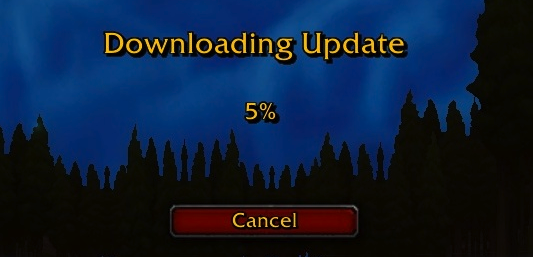
\includegraphics[width=\textwidth]{client_downloading}
	\caption{The \wow client downloading a patch.}
	\label{fig:download}
\end{figure}

\textsc{}\\[1cm]

\textsc{\Large Tutorial}\\[0.5cm]

{ \huge \bfseries Implementing in-client patching for \wow}\\[2cm]


\large \emph{\glqq{}stoneharry\grqq{}}

\large Bernd \emph{\glqq{}schlumpf\grqq{}} \textsc{L\"orwald}

\vfill

% Bottom of the page
{\large \today}

\end{center}

\end{titlepage}

\section{What is this tutorial about?}

This tutorial allows you to use the built-in \wow updating functionality, so that you can send custom patches to the client based on their client version. This is shown in figure \ref{fig:download}.

\section{How to construct a patch}

The patching process allows you to simply send a \mpq file to the client, which can include arbitrary files and a list of commands being executed as soon as the \mpq is downloaded called \file{prepatch.lst}

Typically, such a \mpq file includes a binary \file{installer.exe} to be executed as well as a \file{prepatch.lst} file saying 
\begin{lstlisting}
delete some_no_longer_needed_file
extract some_new_file
extract installer.exe
execute installer.exe
\end{lstlisting}

This extracts the updater, and then runs it. The updater handles the updating process and then deleting the \file{wow-patch.mpq}. \file{wow-patch.mpq} is what the client calls the \mpq file downloaded from the server,  and is checked for and ran if found upon logging in.

The \file{prepatch.lst} can include the commands
\begin{itemize}
	\item \cmd{execute}, which executes an arbitrary file given.
	\item \cmd{extract}, which extracts a file from the \mpq.
	\item \cmd{delete}, which deletes the named file.
\end{itemize}
The file needs to be saved with windows-style line endings (\textbackslash r\textbackslash n). Each line can be at most \np{260} characters long.

\section{Sending the client the patch.}

When logging into the server, the server receives the client's build number. Depending on the client's build, it is able to do different things.

You need to make it so that if the client build is lower or equal to \np{12340} (patch \np{3}.\np{3}.\np{5}a), the server will check for updates, and send them to the client.

The patching process works by the patch being selected, and then the server telling the client that it is about to send a patch and how big the patch is. The client accepts this, and tells the server where to start sending from  -- the full patch if not started being sent before. This means that if the client is disconnected during the transfer for whatever reason, it can resume from where it left off. The server will keep sending \np[byte]{1500} chunks of the patch until the client has the full patch. The client will thus have a \file{wow-patch.mpq} in the \wow directory now, and when the \cmd{restart} button is pressed it will try to open it and execute the contained \file{prepatch.lst}.

The source file modifications required to get this process to work on server side are listed below:

\subsection{ArcEmu}

All of the edits described below take place in the ArcEmu-Logonserver project.

In \file{main.cpp} we have this code snippet:
\lstinputlisting[caption={}]{arcemu_main_loop.cpp}

Each second this code snippet is called. We are interested in line \np{16}. A job is created when a patch is sending. Using this code, it would send \np{1500} bytes (\np{1} chunk) each second. This would take a very, very long time to send \np[MB]{100}. By reducing the sleep time you can make it so that it sends at a much faster rate. You would have to increase the wait time on the other checks by adding to the \% value checks.

A much more efficient way to handle it would be to add the UpdateJobs check to a new thread. However, in reality the logonserver uses very, very little CPU and most machines can run this without any issues, which is bad logic but is a quick implementation:
\lstinputlisting[caption={}]{arcemu_main_loop_scaled.cpp}


The following code snippet from \file{AuthSocket.cpp} shows how the patch is selected for the client:
\lstinputlisting[caption={}]{arcemu_patch_check.cpp}
The logic is that if the client version is less than the server version, then to find the patch for the client. If the patch is found, then to send it to them, else to return a wrong build error.

In ArcEmu the patches are formatted with the pattern \file{LocaleBuild.mpq}. These go in a folder called \file{ClientPatches/} in the same folder as your world executable. For example, for a enGB client running the build  \np{12340} (patch \np{3}.\np{3}.\np{5}a) that you would like to update, you would name the patch \file{enGB12340.mpq}.

The next change happens in \file{AutoPatcher.cpp}: Replace the whole method named \lstinline{Patch * PatchMgr::FindPatchForClient(uint32 Version, const char * Locality)} with the following listing. You will also need to correct the header file to match the new signatures. Also, you need to add a call to \lstinline{InitializePatchList()} to \lstinline{PatchMgr::PatchMgr()}.

\lstinputlisting[caption={Corrected version of Patch* PatchMgr::FindPatchForClient()}]{arcemu_patch_for_client.cpp}

This changes it so that upon this function being called, it gets the correct patch and returns it.

Next go to the function \lstinline{bool PatchMgr::InitiatePatch(Patch * pPatch, AuthSocket * pClient)} and remove the last assignment in the line \lstinline{init.name[0] = 'P'; init.name[1] = 'a'; init.name[2] = 't'; init.name[3] = 'c'; init.name[4] = 'h'; init.name[5] = '\0';}, so that it becomes
\begin{lstlisting}
init.name[0] = 'P';
init.name[1] = 'a';
init.name[2] = 't';
init.name[3] = 'c';
init.name[4] = 'h';
\end{lstlisting}

Inside \file{AutoPatcher.cpp}, you also find this definition, which has the size of \lstinline{char name[];} off by one. Correct the size to be \np{5} instead of \np{6}.
\begin{lstlisting}
struct TransferInitiatePacket
{
	uint8 cmd;
	uint8 strsize;
	char name[6];
	uint64 filesize;
	uint8 md5hash[MD5_DIGEST_LENGTH];
};
\end{lstlisting}

Some of the code above might not work on other platforms than Windows. You may want to adjust it where needed.

\subsection{TrinityCore}

A patch for TrinityCore is provided by schlumpf \href{http://pastebin.com/0BwqxVGf}{here}. It was based on an older version, so you might need to adjust parts of it.

\section{Patching the client to verify the patch}

For the client to verify and attempt to install a patch, you would have to sign your patch with \blizzard's private key, which is sadly non-public. Therefore you need to disable the client verifying that the patch is signed by \blizzard. The following code is for the OSX version of \wow Mists of Pandaria, so your experience on Windows will differ.

As soon as you click the \cmd{restart} button after downloading the patch, the code seen in listing \ref{code:patchdownloadapply} gets executed. As you can see, the part responsible for failing is in line \np{17} to \np{21}. If \lstinline{SFileAuthenticateArchiveEx()} returns a value of \lstinline{authresult} less or equal to \np{4}, patching will be aborted. Therefore, one needs to either change the \lstinline{if} to always be true and therefore be executing the patch, or \lstinline{SFileAuthenticateArchiveEx()} to always verify the archive. You can do the latter either by changing modulus and exponent to your own ones -- which would be good, seeing as your client can't be hijacked by others than and be forced to execute malicious patches -- or by changing \lstinline{SFileAuthenticateArchiveEx()} which only is a wrapper for \lstinline{Blizzard::Mopaq::SFileAuthenticateArchiveEx()}, which sets up a RSA / SHA-1 signature structure which is then comparing the actual signature of the \mpq with the signature in the given \file{signaturefile}.

Changing \lstinline{SFileAuthenticateArchiveEx()} instead of \lstinline{CGlueMgr::PatchDownloadApply()} has the advantage of also enabling custom surveys, which can be streamed to the user on login and should therefore be chosen to be patched. You can see the C++ version of  \lstinline{SFileAuthenticateArchiveEx()} in listing \ref{code:SFileAuthenticateArchiveEx} and the assembler version in  listing \ref{code:SFileAuthenticateArchiveExASM}. As you easily can see, the \lstinline{if} needs to be removed and \lstinline{*authresult = authresult_temp;} needs to be changed into \lstinline{*authresult = 5;}. As it is easier just rewriting that function than modifying it, I suggest patching it to be looking as seen in listings \ref{code:auth_fixed} and  \ref{code:auth_fixed_asm}.

\lstinputlisting[label=code:patchdownloadapply, caption={void CGlueMgr::PatchDownloadApply()}]{CGlueMgr__PatchDownloadApply.cpp}

\lstinputlisting[label=code:SFileAuthenticateArchiveEx,caption={bool SFileAuthenticateArchiveEx()}]{SFileAuthenticateArchiveEx.cpp}
\lstinputlisting[language={[x86masm]Assembler},label=code:SFileAuthenticateArchiveExASM,caption={Assembler version of bool SFileAuthenticateArchiveEx()}]{SFileAuthenticateArchiveEx.asm}

\lstinputlisting[label= code:auth_fixed,caption={proposed patch  for bool SFileAuthenticateArchiveEx()}]{SFileAuthenticateArchiveEx_fixed.cpp}
\lstinputlisting[language={[x86masm]Assembler},label= code:auth_fixed_asm,caption={Assembler version of proposed patch  for bool SFileAuthenticateArchiveEx()}]{SFileAuthenticateArchiveEx_fixed.asm}

\section{Applying the patch}

The executable run from the \mpq is where you update the client. Myself, I wrote a quick application in C++ that renames the \file{WoW.exe} (as a backup) then writes files from the \file{wow-patch.mpq} into a \file{patch.mpq} and deletes the \file{Cache/} folder as well as the \file{wow-patch.mpq}. It also writes a new executable \file{WoW.exe}, which has an updated build number and then starts the new \file{WoW.exe}. Now the client should be fully up to date and be accepted by your server's check and proceed to log in without additional patching.

\section{Updating the client version}

There are different locations, where the build number is referenced in the client. There is a string variant to be written onto the login screen. This one is supplied by \lstinline{int Script_GetBuildInfo(lua_State *)}. You can easily find the location to modify via just searching for the number given on the login screen as string. You will come up with two locations: One where the build number is stored and another one where the version as well as build-date is. These are all only for logging and to show the user which version he has and should be set by you to help the user identify the version. The actually relevant build number for patching is in \lstinline{RealmConnection::HandleAuthChallenge()}.

Offsets specific to build \np{12340} (patch \np{3}.\np{3}.\np{5}a) can be found \href{http://www.ownedcore.com/forums/general/programming/326606-wow-exe-custom-build.html}{on OwnedCore}.

I would always advise making a back up of your WoW executable before attempting to modify anything. You should use incrementing numbers above \np{12340}, to be able to supply incremental patches. Every patch should have a different build number, of course.

\end{document}
